\begin{usecase}{Add Event Manually}
    \ucbasicinfo{High}{Regular}
    \ucshortdescription{This UC allows users to add events manually.}
    \uctrigger{The user clicks add event manually icon or a date on the calendar and adds the events.}
    \ucactors{User}{None}
    \ucpreconditions{The user is logged into the application.}
    \ucrelationships{Suggest Conflict Resolutions}{N/A}{N/A}
    \ucinputsoutputs{
      \begin{itemize}
        \item \textbf{Event Name} (Source: User)
        \item \textbf{Event Location} (Source: User)
        \item \textbf{Is all day?} (Source: User)
        \item \textbf{Event Date (Start and End)} (Source: User)
        \item \textbf{Event Time (Start and End)} (Source: User)
        \item \textbf{Event Description} (Source: User)
        \item \textbf{Notifications/Reminders} (Source: User)
      \end{itemize}
    }{
      \begin{itemize}
        \item \textbf{New Calendar event}
         (Destination: Calendar)
      \end{itemize}
    }
    \ucmainflow{
      \begin{enumerate}
        \item The user clicks the add event manually icon or a date on the calendar.  
          \ucinfo{The add event manually form is displayed.}
        \item The user sets the details of the event in the respective fields and saves the event. 
          \ucinfo{The event is displayed on the calendar with its details.}
      \end{enumerate}
    }
    \ucalternateflows{
      \begin{enumerate}
        \item If the validation fails the user can try again afte fixing the issues
      \end{enumerate}
    }
    \ucexceptions{
      \begin{itemize}
        \item The end time is before the start time.
        \item The user attempts to save the event without filling in mandatory fields.
      \end{itemize}
    }
    \ucconclusion{The UC ends when the event has been successfully added to the calendar, and displayed.}
    \ucpostconditions{The event is successfully added to the calendar and displayed in the correct time slot.}
    \ucspecialrequirements{The interface must be simple and allowing users to input events with less efforts.}
\end{usecase}

\begin{figure}[!h]
  \centering
  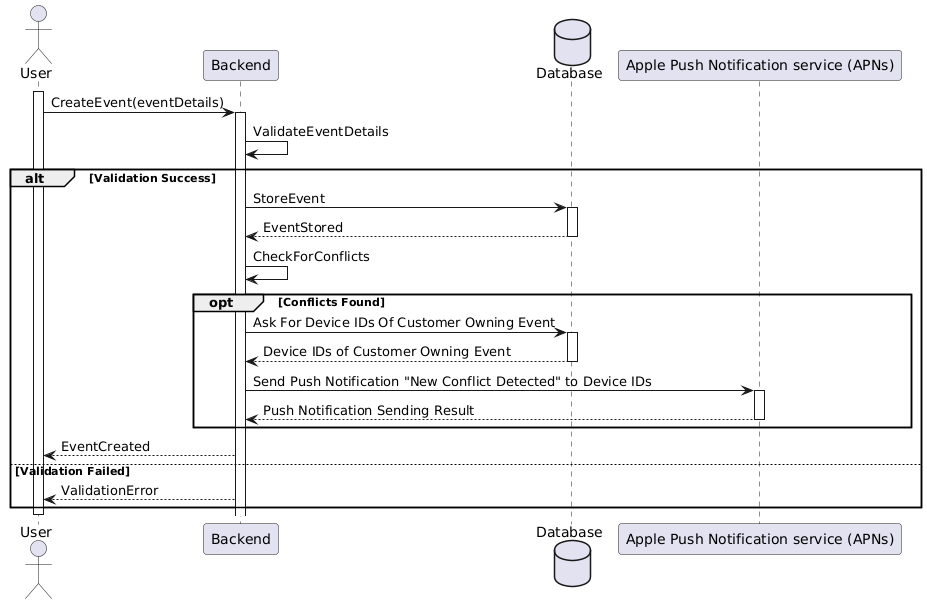
\includegraphics[width=\textwidth]{images/docs/diagrams/sequence-diagrams/all-sequence-diagrams/Add Event Manually.png}
  \caption{Add Event Manually Sequence Diagram}
  \label{fig:seq/add-event-manually}
\end{figure}